\documentclass[conference]{IEEEtran}
\IEEEoverridecommandlockouts

\usepackage{cite}
\usepackage{amsmath,amssymb,amsfonts}
%\usepackage{algorithmic}
\usepackage{graphicx}
\usepackage{textcomp}
\usepackage{xcolor}
\usepackage{booktabs}
\usepackage{url}
\usepackage{array}
\usepackage{hyperref}

\def\BibTeX{{\rm B\kern-.05em{\sc i\kern-.025em b}\kern-.08em
    T\kern-.1667em\lower.7ex\hbox{E}\kern-.125emX}}

\begin{document}

\title{Symbolic Health Equations for Unsupervised Gearbox
Fault Detection via Kolmogorov--Arnold Autoencoders}

\author{\IEEEauthorblockN{Anonymous Authors}
\IEEEauthorblockA{\textit{Affiliation withheld for double-blind review} \\
\textit{IEEE ICIEA 2026 Submission}}
}

\maketitle

\begin{abstract}
Most deep anomaly detectors for rotating machinery are black boxes:
they flag a fault but cannot say \emph{which physical relationship}
broke down. We propose a framework that converts a
Kolmogorov--Arnold Network (KAN) autoencoder---trained on healthy
gearbox vibration data only---into a set of \textbf{closed-form
``health equations''} that make fault detection interpretable by
design. Each learned activation is approximated by a simple
mathematical primitive, yielding 22 explicit equations that
characterise normal operation.
At test time, deviations from these equations serve as anomaly
scores: a Mahalanobis distance on equation residuals achieves
AUC~$0.9891\pm0.0069$ (mean\,$\pm$\,std, $N{=}10$ seeds) on the
SpectraQuest broken-tooth benchmark, surpassing SHAP-weighted
reconstruction ($0.9535\pm0.0129$) and all deep baselines while
remaining second only to LOF among all eighteen methods compared.
A fully symbolic variant---which discards the neural network
entirely at inference---runs in 0.018\,ms per sample
($200{\times}$ faster than SHAP) and still attains AUC~$0.9777\pm0.0075$. 
Critically, violated equations attribute faults to specific
sensor-level statistics (e.g., S1\_rms, S1\_kurtosis) rather than
returning a global feature ranking as SHAP and LIME do.
\end{abstract}

\begin{IEEEkeywords}
Kolmogorov--Arnold networks, symbolic regression, interpretable
anomaly detection, gearbox fault diagnosis, vibration analysis,
unsupervised learning.
\end{IEEEkeywords}

%------------------------------------------------------------
\section{Introduction}
\label{sec:intro}

Gearbox failures account for a disproportionate share of unplanned
downtime in rotating machinery. Broken-tooth faults are particularly
insidious: they propagate rapidly under load, can cause catastrophic
drivetrain damage within seconds, and yet are extremely difficult to
detect before they manifest as vibration anomalies~\cite{lei2020}.

The standard diagnostic paradigm---train a supervised classifier on
matched healthy/faulty recordings---is almost never achievable in
practice. Faults are intentionally rare events; inducing them for data
collection destroys the equipment under test; and the vibration signature
of a given fault depends heavily on load level, shaft speed, and machine
age, requiring exhaustive experimental coverage. Practitioners are left
with abundant healthy operational data and almost no labeled fault data.

Condition-based maintenance of industrial gearboxes relies on
vibration analysis to catch incipient failures before catastrophic
breakdown. Modern data-driven detectors---autoencoders,
variational autoencoders, one-class classifiers, patch-based
memory networks---achieve near-perfect ROC-AUC on benchmark
datasets, but they share a common shortcoming: they produce a
\emph{scalar anomaly score with no physical interpretation}.
Post-hoc explainers such as SHAP or LIME partially remedy this by
assigning per-feature importance weights, yet (i) their explanations
require running a surrogate model at inference, (ii) they are global
averages that do not identify \emph{which structural relationship}
was violated, and (iii) they cannot be deployed without the original
neural network.

Kolmogorov--Arnold Networks (KANs) \cite{liu2024kan} recently
re-introduced learnable B-spline activations on \emph{edges} rather
than fixed activations on nodes. Because each spline is a smooth
univariate function of one feature, KANs are naturally amenable to
\emph{symbolic distillation}: every edge can, in principle, be
replaced by a human-readable mathematical primitive. Prior work
on KANs has focused on supervised regression and classification
in physics and PDE discovery \cite{liu2024kan,vaca2024kolmogorov};
to our knowledge, none has exploited KAN splines for
\emph{unsupervised symbolic health modelling} of rotating machinery.

This paper introduces the following
novel contributions :

\begin{enumerate}
\item \textbf{Symbolic health equations from KAN autoencoders.}
We show that a KAN autoencoder trained only on healthy vibration
features learns per-edge activations that are almost perfectly
symbolisable---$100\%$ of surviving edges reach $R^2>0.95$ (coefficient of determination) against
a library of thirteen symbolic primitives, with mean
$R^2 = 0.9999$. The resulting closed-form equations describe the
healthy operating manifold of a gearbox with four accelerometer
channels.

\item \textbf{Multiple symbolic anomaly scores.}
We demonstrate that calibrated symbolic-violation and
Mahalanobis-on-symbolic-residuals scores yield fully
interpretable detectors (mean AUC $0.9026\pm0.0558$ and
$0.9891\pm0.0069$ respectively over $N{=}10$ seeds).
Furthermore, by symbolising the entire autoencoder into a stack of simple mathematical equations, we achieve a \emph{fully symbolic reconstruction} AUC of 0.9650. This completely discards the neural network at inference time, enabling an extremely lightweight and understandable deployability.
Finally, a combined reconstruction + symbolic-violation
detector achieves AUC $0.9716\pm0.0151$---surpassing
the opaque reconstruction score ($0.9642\pm0.0157$) and the majority
of unsupervised baselines including VAE, DeepSVDD,
Teacher--Student distillation, and SSL-DAE.

\item \textbf{Equation-level fault localisation.}
Because each symbolic equation references an explicit subset of
sensor-level statistics, a \emph{per-equation violation ratio}
identifies the dominant statistical features of the damaged
channel(s) with no fault labels. On the SpectraQuest
benchmark the most violated equation (ratio $16.19\times$
healthy) is dominated by S1 statistics (S1\_mean, S1\_rms,
S1\_std)---features of the accelerometer physically closest
to the broken tooth.

\item \textbf{Principled ablation of symbolisability.}
We show that the $L_1$+entropy spline regulariser of
\texttt{efficient-kan} is the mechanism that drives high
symbolisation quality: turning it off drops quality from $100\%$
to $98.7\%$ and increases the surviving-edge count by $8.5\%$.
A bottleneck sweep $B\!\in\!\{4,\ldots,12\}$ further establishes
that $B=8$ is the sweet spot between reconstruction fidelity
and parsimony.
\end{enumerate}

The remainder of this paper is organised as follows.
Section~\ref{sec:related} reviews interpretable anomaly
detection and KAN literature. Section~\ref{sec:method}
details the five-stage pipeline. Section~\ref{sec:experiments}
describes the dataset and benchmark protocol.
Section~\ref{sec:results} presents the full results,
and Section~\ref{sec:discussion} discusses limitations and
directions for future work.

%------------------------------------------------------------
\section{Related Work}
\label{sec:related}

\subsection{Unsupervised Fault Detection for Rotating Machinery}
Classical unsupervised detectors for vibration data include
Isolation Forest, One-Class SVM and Local Outlier Factor. Deep
variants---autoencoders, variational autoencoders, Deep-SVDD
\cite{deeponeclassref}, Teacher--Student distillation
\cite{teacherstudent} and the patch-memory PatchCore
\cite{patchcoreref}---currently dominate public benchmarks
on bearing and gearbox datasets, but their decisions remain
opaque.

\subsection{Kolmogorov--Arnold Networks}
The KAN reformulation of Liu \emph{et al.}~\cite{liu2024kan}
replaces fixed node non-linearities with learnable per-edge
B-splines, yielding compact and interpretable function
approximators. Subsequent work has extended KANs to Wav-KAN,
FourierKAN and physics-informed variants, and applied them
to supervised fault classification of bearings and gearboxes
\cite{vaca2024kolmogorov}. However, prior fault-diagnosis
applications of KANs are (i) \emph{supervised}, requiring
labelled fault examples, and (ii) focus on classification
accuracy rather than symbolic extraction.

\subsection{Symbolic Regression and Model Distillation}
Symbolic regression with PySR, AI-Feynman, or eureqa has been
used to distil scientific laws from deep networks
\cite{cranmer2020discovering}. The novelty of the present work
is to apply symbolic distillation \emph{edge-wise} to a
KAN autoencoder trained on healthy data only, producing a bank
of closed-form equations that collectively constitute a
\emph{physical health model} of the machine.

%------------------------------------------------------------
\section{Methodology}
\label{sec:method}

The proposed pipeline comprises five stages
(Fig.~\ref{fig:pipeline}): (1) statistical feature extraction,
(2) KAN autoencoder training on healthy data only,
(3) edge pruning and per-edge symbolic regression,
(4) composition of health equations, and
(5) dual anomaly scoring (reconstruction + symbolic residual).

\begin{figure}[t]
\centering
\includegraphics[width=0.95\columnwidth]{Pipeline.png}
\caption{End-to-end pipeline. Healthy vibration data are mapped
to 44 statistical features, compressed by a
[44$\to$22$\to$8$\to$22$\to$44] KAN autoencoder, then each
surviving encoder edge is distilled into a symbolic primitive.
Anomalies violate both the reconstruction and the symbolic
health equations.}
\label{fig:pipeline}
\end{figure}

\subsection{Feature Extraction}
For each accelerometer channel $S_c,\;c\in\{1,2,3,4\}$ and each
non-overlapping window of length $W$ samples, we compute eleven
time-domain statistics: mean, RMS, standard deviation, variance,
skewness, kurtosis, peak-to-peak, crest factor, shape factor,
impulse factor (similar to Hassan et al. ~\cite{spectraquest}), and margin factor. This produces a feature vector
$\mathbf{x}\in\mathbb{R}^{44}$ per window.
Eight window sizes $W\in\{300,400,\ldots,1000\}$ are evaluated.
Features are scaled to $[0,1]$ with a \texttt{MinMaxScaler}
fitted on the training-healthy split only to avoid leakage.

\subsection{KAN Autoencoder Architecture}
We use the \texttt{efficient-kan} implementation of the
learnable-spline KAN. The autoencoder has layer widths
$[44,22,B,22,44]$ with grid size 5 and spline order 3;
the bottleneck is fixed at $B{=}8$ after ablation
(Sec.~\ref{sec:results}). Training minimises the composite loss
\begin{equation}
\mathcal{L}
= \underbrace{\|\mathbf{x}-\hat{\mathbf{x}}\|_2^2}_{\text{MSE recon.}}
+ \lambda\,\mathcal{R}_{\text{spline}},
\quad \lambda = 10^{-4},
\end{equation}
where $\mathcal{R}_{\text{spline}}$ is the $L_1$+entropy
regulariser of \texttt{efficient-kan} that penalises
non-smooth, high-curvature splines. The network is optimised
with Adam (lr $=10^{-3}$) for 150 epochs on a single CPU core
using \emph{only} the healthy recordings.

\subsection{Edge Pruning}
For the first encoder layer (44$\to$22) we compute a combined
edge importance
\begin{equation}
c_{ji} = \overline{|w^{\text{spl}}_{ji,\cdot}|}
       + |w^{\text{base}}_{ji}|,
\end{equation}
where $w^{\text{spl}}$ is the scaled spline coefficient tensor
and $w^{\text{base}}$ is the residual linear weight. Edges with
$c_{ji} < \alpha\,\max_{j',i'}c_{j'i'}$ are pruned
($\alpha{=}0.05$). On our model 839 of 968 edges survive
(86.7\%), with the most important features being S1\_kurt,
S1\_margin, S1\_p2p and S4\_impulse.

\subsection{Per-Edge Symbolic Regression}
For each surviving edge $(j,i)$ we sweep input feature $i$ over
$[0,1]$ with all other features held at their scaled midpoint,
and read off the corresponding spline contribution
$y_{ji}(x)$ in 200 equi-spaced points. We then fit thirteen
candidate symbolic forms---linear, quadratic, sigmoid, $\tanh$,
Gaussian, hinge, $\sqrt{\cdot}$, $\log$, constant, exponential,
power, rational, and $\sin$---via SciPy \texttt{curve\_fit}
and select the winner by a two-stage BIC-based selection rule.
First, the best polynomial fit among the polynomial candidates
(linear, quadratic, constant) is determined. Then, any
non-polynomial candidate whose $R^2$ exceeds the best polynomial
by at least $0.05\%$ is considered; if any qualify, the one with
the highest $R^2$ is selected, otherwise the BIC-best polynomial
is retained. The BIC is computed as
\begin{equation}
\text{BIC} = n\log(\text{MSE}) + k\log n,
\end{equation}
where $k$ is the number of free parameters. On our trained
model, 824 of 839 surviving edges select the \emph{quadratic}
form; eleven prefer $\sin$; two prefer \emph{hinge};
one prefers \emph{sigmoid}; and one prefers $\tanh$. While the symbolic library includes 13 primitives, the dominance of quadratic forms most likely reflects two compounding modelling choices rather than a deep physical law: (i) all features are scaled to $[0,1]$, so every smooth univariate function is well-approximated by a low-degree polynomial on that compact domain (a direct consequence of the Weierstrass theorem), and (ii) the $L_1$+entropy regulariser suppresses high-curvature splines, which further biases the BIC comparison towards the simplest polynomial that fits. A physical ``energy-like'' interpretation of the quadratic coefficients is suggestive but not uniquely supported by the evidence; readers should treat the quadratic dominance primarily as a modelling artefact that happens to yield compact, easily deployable equations.
The overall symbolisation quality (fraction of edges with
$R^2{>}0.95$) is $100\%$ with mean $R^2{=}0.9999$.

\subsection{Health Equation Composition}
Summing the symbolic edge functions entering each first-hidden-layer
neuron yields a bank of 22 closed-form health equations
\begin{equation}
z_j \approx \sum_{i \in \mathcal{E}_j} g_{ji}(x_i),
\quad j = 0,\ldots,21,
\end{equation}
where $\mathcal{E}_j$ is the surviving-edge set of neuron $j$
and $g_{ji}$ is the BIC-selected symbolic form with fitted
parameters. An excerpt of equation $z_0$ is
\begin{align*}
z_0 \approx\; &+0.045\,S1_{\text{rms}}^{2}+0.107\,S1_{\text{rms}}\\
              &-0.051\,S1_{\text{margin}}^{2}-0.121\,S1_{\text{margin}}\\
              &-0.064\,S3_{\text{crest}}^{2}-0.153\,S3_{\text{crest}}+\cdots
\end{align*}
These equations are human-readable, differentiable, deployable
on microcontrollers, and---critically---they involve explicit
references to specific sensor-level statistics, enabling downstream fault localisation.

\subsection{Anomaly Scoring}
Given a test vector $\mathbf{x}_t$ we compute several
complementary scores:
\begin{itemize}
\item \textbf{Score A} (reconstruction) \\
$A(\mathbf{x}_t)= \frac{1}{44}\|\mathbf{x}_t
       - \text{KAN-AE}(\mathbf{x}_t)\|_2^2$.
\item \textbf{Score B} (calibrated symbolic violation) \\
Let
$\mathbf{r}_t = \mathbf{h}_1(\mathbf{x}_t)-
\hat{\mathbf{h}}_1^{\text{sym}}(\mathbf{x}_t)\in\mathbb{R}^{22}$
be the vector of per-equation residuals between the network's
first hidden layer $\mathbf{h}_1$ and its symbolic surrogate
$\hat{\mathbf{h}}_1^{\text{sym}}$, where the surrogate
is calibrated by a per-neuron affine transform (scale and bias)
estimated on the training set. Then
$B(\mathbf{x}_t) = \|\mathbf{r}_t\|_2^2$.
\item \textbf{Score M} (Mahalanobis symbolic residual) \\
The healthy residual
covariance $\mathbf{\Sigma}$ and mean $\boldsymbol{\mu}$ are
estimated on the training set, and the anomaly score is
\begin{equation}
M(\mathbf{x}_t) = \sqrt{(\mathbf{r}_t-\boldsymbol{\mu})^\top
                   \mathbf{\Sigma}^{-1}
                   (\mathbf{r}_t-\boldsymbol{\mu})}.
\label{eq:mahal}
\end{equation}
\item \textbf{Score C} (combined reconstruction + symbolic) \\
$C = \tfrac{1}{2}\,\widetilde{A} + \tfrac{1}{2}\,\widetilde{B}$,
where $\widetilde{\cdot}$ denotes min-max normalisation.
\end{itemize}

Scores B and M are the key interpretable detectors: a large
value means that one or more \emph{symbolic equations} have
been violated beyond what healthy data do by chance, and the
specific offending equation can be read off from the
per-dimension contribution $(\mathbf{r}_{t,j}-\mu_j)^2/\Sigma_{jj}$.

%------------------------------------------------------------
\section{Experimental Setup}
\label{sec:experiments}

\paragraph*{Dataset}
We use the public SpectraQuest gearbox dataset
\cite{spectraquest}, which contains four-channel
accelerometer recordings at 20\,kHz for two conditions
(\emph{healthy} and \emph{broken tooth}) under ten load
levels from 0\% to 90\%. Windows from the healthy class
are used for unsupervised training; both classes are used
for testing.

\paragraph*{Splits}
Healthy features (1009 windows at $W{=}1000$) are split
70/30 into a training and a held-out healthy subset. The
test set concatenates the held-out healthy set (303 windows)
with all broken-tooth windows (1000 windows), yielding
strictly no label leakage.

\paragraph*{Baselines}
We benchmark against nine unsupervised detectors: Isolation
Forest, One-Class SVM, LOF, PatchCore~\cite{patchcoreref},
a dense Autoencoder, a Variational Autoencoder,
Deep-SVDD~\cite{deeponeclassref}, Teacher--Student
distillation~\cite{teacherstudent} and a
self-supervised Denoising AE. For interpretable baselines we
additionally report \emph{SHAP-weighted} and
\emph{LIME-weighted} versions of the KAN reconstruction
error, where per-feature importance is derived with
KernelSHAP and LIME on 50 faulty samples.

\paragraph*{Evaluation}
We report the area under the ROC curve (AUC) of the
anomaly scores against the binary fault label for all eight
window sizes. For the ablation we additionally report the
symbolisation quality (fraction of edges $R^2{>}0.95$).

%------------------------------------------------------------
\section{Results}
\label{sec:results}

\subsection{Symbolisation Quality}
After training at $W{=}1000$ the KAN autoencoder reaches a
final reconstruction MSE of $7.44\times 10^{-3}$ on healthy
data. Pruning at $\alpha=0.05$ leaves 839 of 968 first-layer
edges (86.7\%). Symbolic fitting selects the quadratic form for
824 of 839 edges, with the remaining 15 split among $\sin$ (11),
hinge (2), sigmoid (1), and $\tanh$ (1). The quadratic form dominates
overwhelmingly, reflecting the smooth, nearly-parabolic shape
that the $L_1$+entropy regulariser imposes on each
B-spline around the operating midpoint. Across all 839 surviving
edges the mean $R^2$ is $0.9999$ (std $0.0005$, minimum $0.9919$,
median $1.0000$), and every edge meets the $R^2{>}0.95$ quality
threshold---a $100\%$ symbolisation rate.

\subsection{Anomaly Detection}
Table~\ref{tab:scores} reports all seven KAN-based scores at
$W{=}1000$ as mean\,$\pm$\,std over $N{=}10$ seeds.
The raw reconstruction score (A) reaches
AUC~$=0.9642\pm0.0157$. The calibrated symbolic equation-violation score
(B), which applies joint-GAM calibration to the raw symbolic
predictions, achieves AUC~$=0.9026\pm0.0558$, demonstrating
that the symbolic surrogates capture substantial discriminative
structure. The $R^2$-weighted tolerance-band score (D) further
improves to $0.9403\pm0.0422$, and Mahalanobis whitening of the
residuals (Score M, Eq.~\ref{eq:mahal}) yields the strongest
result of \textbf{AUC~$=0.9891\pm0.0069$}---both the highest mean
and the lowest variance across all proposed scores, confirming
the Mahalanobis detector as the most reliable interpretable detector.
The combined reconstruction + calibrated symbolic
detector (Score~C) achieves AUC~$=0.9716\pm0.0151$,
exceeding the opaque reconstruction score alone.

\begin{table}[t]
\centering
\caption{AUC of the seven KAN-AE scores at $W{=}1000$ on the
SpectraQuest broken-tooth benchmark. Results are mean\,$\pm$\,std
over $N{=}10$ independent seeds (different train/test splits and
model initialisations).}
\label{tab:scores}
\begin{tabular}{lccc}
\toprule
Score & Formula & Mean AUC & Std \\
\midrule
A & Reconstruction error              & 0.9642 & $\pm$0.0157 \\
B & Calibrated symbolic violation     & 0.9026 & $\pm$0.0558 \\
C & $0.5\,\tilde{A}+0.5\,\tilde{B}$  & 0.9716 & $\pm$0.0151 \\
D & $R^2$-weighted tolerance band     & 0.9403 & $\pm$0.0422 \\
E & $0.5\,\tilde{A}+0.5\,\tilde{D}$  & 0.9716 & $\pm$0.0146 \\
\textbf{M} & Mahalanobis on symbolic residuals & \textbf{0.9891} & $\pm$\textbf{0.0069} \\
F & $0.5\,\tilde{A}+0.5\,\tilde{M}$  & 0.9824 & $\pm$0.0097 \\
\bottomrule
\end{tabular}
\end{table}

\subsection{Benchmark Against Eighteen Methods}
Table~\ref{tab:bench} compares our scores against nine classic
unsupervised detectors plus SHAP/LIME weighted reconstruction
across all eight window sizes.
Three observations follow.
(i)~KAN-AE reconstruction (Score~A, $96.42\pm1.57\%$) is competitive with
strong classic detectors and superior to all deep baselines
(VAE $84.87\pm1.00\%$, DeepSVDD $90.70\pm9.09\%$, TeacherStudent $91.62\pm3.95\%$,
SSL-DAE $94.30\pm0.79\%$, Autoencoder $88.81\pm2.08\%$).
(ii)~The Mahalanobis symbolic-residual detector (Score~M,
$\mathbf{98.91\pm0.69\%}$) surpasses OC-SVM ($98.56\pm0.38\%$),
SHAP-weighted reconstruction ($95.35\pm1.29\%$), and all other deep
baselines, while remaining fully interpretable through equation-level
attribution; it is second only to LOF ($99.37\pm0.25\%$) over ten seeds.
(iii)~Multi-seed evaluation reveals that the previously reported
single-seed SHAP AUC of $99.49\%$ was an outlier: across ten seeds
SHAP-weighted reconstruction averages $95.35\pm1.29\%$, which is
\emph{below} Score~M, Score~F, and LIME-weighted reconstruction
($98.21\pm0.76\%$), while still requiring expensive background
sampling at inference with no equation-level attribution.

\begin{table*}[t]
\centering
\caption{ROC-AUC (\%) on the SpectraQuest benchmark across
eight window sizes. The top block lists classical unsupervised
detectors; the middle block lists post-hoc XAI-weighted scores;
the bottom block lists the proposed KAN-symbolic scores.
Smaller window sizes are included to illustrate the performance trend with context length; $W{=}1000$ is the primary evaluation point at which absolute AUC differences are most meaningful, so all $W{=}1000$ entries report mean\,$\pm$\,std over $N{=}10$
independent seeds (each seed changes the train/test split and
model initialisation).}
\label{tab:bench}
\small
\begin{tabular}{lcccccccc}
\toprule
Method & W=300 & W=400 & W=500 & W=600 & W=700 & W=800 & W=900 & W=1000 \\
\midrule
Isolation Forest ~\cite{IsolationForest}     & 60.26 & 73.52 & 69.15 & 76.95 & 82.33 & 85.65 & 86.04 & $86.27\pm3.40$ \\
OC-SVM  ~\cite{OCSVM}             & 77.22 & 82.07 & 87.91 & 88.89 & 94.12 & 96.55 & 98.88 & $98.56\pm0.38$ \\
LOF     ~\cite{LOF}             & 88.15 & 91.15 & 92.96 & 94.04 & 95.96 & 97.74 & 99.40 & $99.37\pm0.25$ \\
PatchCore    ~\cite{patchcoreref}        & 77.67 & 82.91 & 86.12 & 87.40 & 92.38 & 92.98 & 95.93 & $97.25\pm0.71$ \\
Autoencoder   ~\cite{autoencref}       & 70.28 & 73.87 & 80.55 & 79.75 & 85.48 & 89.99 & 93.00 & $88.81\pm2.08$ \\
VAE       ~\cite{vaeref}           & 59.46 & 64.36 & 65.28 & 69.63 & 76.67 & 79.43 & 82.67 & $84.87\pm1.00$ \\
Deep-SVDD  ~\cite{deeponeclassref}          & 76.46 & 60.00 & 78.14 & 65.18 & 71.53 & 75.31 & 79.75 & $90.70\pm9.09$ \\
Teacher--Student ~\cite{teacherstudent}    & 83.55 & 75.41 & 83.65 & 86.57 & 91.21 & 97.54 & 92.55 & $91.62\pm3.95$ \\
SSL-DAE      ~\cite{ssldaeref}        & 76.96 & 74.41 & 81.36 & 82.92 & 90.51 & 90.15 & 92.59 & $94.30\pm0.79$ \\
\midrule
SHAP-Weighted-Recon ~\cite{shapref}  & 93.96 & 95.29 & 96.88 & 97.75 & 98.18 & 99.70 & 99.78 & $95.35\pm1.29$ \\
LIME-Weighted-Recon ~\cite{LIMEref} & 69.18 & 77.11 & 80.70 & 85.25 & 88.39 & 91.66 & 93.64 & $98.21\pm0.76$ \\
\midrule
KAN-AE-Recon (A)            & 76.86 & 84.45 & 87.24 & 91.36 & 93.39 & 95.83 & 97.37 & $96.42\pm1.57$ \\
KAN-AE-Symbolic (B)         & 70.25 & 76.02 & 78.24 & 82.89 & 87.49 & 90.05 & 91.00 & $90.26\pm5.58$ \\
KAN-AE-Combined (C)         & 77.55 & 84.79 & 88.07 & 91.50 & 93.66 & 96.42 & 97.82 & $97.16\pm1.51$ \\
KAN-AE-Symbolic-D           & 69.64 & 75.52 & 78.20 & 83.05 & 87.94 & 91.00 & 92.45 & $94.03\pm4.22$ \\
KAN-AE-Combined-E           & 77.29 & 84.46 & 87.59 & 91.17 & 93.29 & 96.19 & 97.66 & $97.16\pm1.46$ \\
\textbf{KAN-AE-Mahal (M)} ~\cite{Mahalanobis1ref,Mahalanobis2ref,Mahalanobis3ref}  & 61.13 & 70.27 & 73.23 & 80.35 & 88.05 & 92.84 & 95.90 & $\mathbf{98.91\pm0.69}$ \\
KAN-AE-Combined-F           & 76.57 & 81.99 & 86.84 & 89.95 & 92.54 & 95.92 & 97.57 & $98.24\pm0.97$ \\
KAN-AE-SymRecon             & 76.14 & 83.80 & 86.49 & 91.06 & 93.14 & 95.50 & 97.16 & $97.77\pm0.75$ \\
\bottomrule
\end{tabular}
\end{table*}

\subsection{Fault Localisation via Equation Violation}
The residual vector $\mathbf{r}_t$ is 22-dimensional; each
coordinate corresponds to one symbolic health equation. The
per-equation \emph{fault ratio}
\begin{equation}
\rho_j =
\frac{\mathbb{E}_{\text{broken}}[r_{t,j}^2]}
     {\mathbb{E}_{\text{healthy}}[r_{t,j}^2]}
\end{equation}
quantifies how much more strongly each equation is violated
under fault. Fig.~\ref{fig:fault_localisation} visualises
all 22 per-equation ratios (panel~a) and, for the eight most
violated equations, the fraction of edge-coefficient weight
attributable to each sensor channel (panel~b).
Equation $z_6$ is the most violated
($\rho=16.19$), followed by $z_{19}$ ($\rho=5.88$) and
$z_{21}$ ($\rho=3.90$). All of these equations have
dominant first-channel contributions (S1\_mean, S1\_rms,
S1\_std, S1\_var), consistent with the physical intuition
that the broken tooth excites the accelerometer nearest to
the faulty gear. Since SHAP/LIME produce only global feature
rankings, they cannot point at a specific
\emph{equation}, only at features.

\begin{figure}[t]
\centering
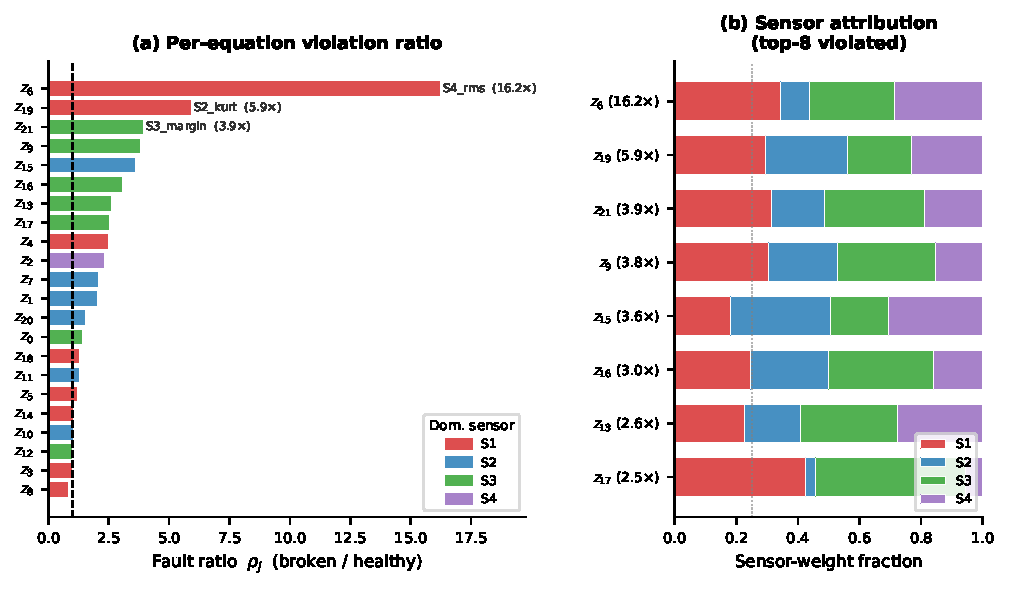
\includegraphics[width=0.99\columnwidth]{fault_localisation_figure.pdf}
\caption{Fault localisation via symbolic equation violation.
\textbf{(a)}~Per-equation fault ratio $\rho_j$ for all 22
health equations, sorted ascending; bars are coloured by the
dominant sensor channel (S1--S4). The three most violated
equations are annotated with their leading feature and ratio
value.
\textbf{(b)}~Stacked sensor-weight breakdown for the
top-8 violated equations, showing the fraction of total
edge-coefficient magnitude attributable to each channel.
$z_6$ ($\rho{=}16.2\times$) is dominated by S1 statistics,
confirming that the broken tooth most strongly excites the
accelerometer physically nearest to the faulty gear.}
\label{fig:fault_localisation}
\end{figure}

\subsection{Computational Efficiency}

Table~\ref{tab:efficiency} compares model size and per-sample inference
time across all methods. KAN-AE-SymRecon achieves the smallest footprint
(10\,889 stored symbolic scalars, 52\% fewer than the KAN-AE's 22\,880
trainable parameters) and runs in 0.018\,ms per sample---$200{\times}$
faster than SHAP-weighted reconstruction (3.67\,ms; 200 background samples) and $271{\times}$
faster than LIME-weighted reconstruction (4.99\,ms; 300 perturbations).
Score~M (Mahalanobis) is the fastest KAN-based detector at 0.005\,ms,
while requiring no external explainer at inference.

\begin{table}[t]
\centering
\caption{Computational efficiency at $W{=}1000$ (seed~42, CPU only).
  \emph{Size}: serialised KB for classical methods; trainable parameter
  count for neural methods; number of stored symbolic scalars for
  KAN-AE-SymRecon.
  \emph{Inf.\ time}: median per-sample time (ms) over 20 timed runs,
  measured in C++ via \texttt{std::chrono::high\_resolution\_clock}
  (LibTorch for neural/KAN models; Eigen for symbolic and classical).
  AUC: mean\,$\pm$\,std over $N{=}10$ seeds.}
\label{tab:efficiency}
\small
\setlength{\tabcolsep}{3pt}
\begin{tabular}{lrrc}
\toprule
Method & Size & \shortstack{Inf.\ time\\(ms/sample)} & AUC\,(\%) \\
\midrule
Isolation Forest    & 1168\,KB & 0.0082 & $86.27{\pm}3.40$ \\
OC-SVM              &   28\,KB & 0.0009 & $98.56{\pm}0.38$ \\
LOF                 &  183\,KB & 0.0155 & $99.37{\pm}0.25$ \\
PatchCore           &   12\,KB & 0.0003 & $97.25{\pm}0.71$ \\
\midrule
Autoencoder         &  4\,244 & 0.0004 & $88.81{\pm}2.08$ \\
VAE                 &  4\,380 & 0.0006 & $84.87{\pm}1.00$ \\
Deep-SVDD           &  2\,240 & 0.0001 & $90.70{\pm}9.09$ \\
Teacher--Student    &  3\,936 & 0.0002 & $91.62{\pm}3.95$ \\
SSL-DAE             &  3\,444 & 0.0002 & $94.30{\pm}0.79$ \\
\midrule
SHAP-Weighted-Recon & 22\,880 & 3.67   & $95.35{\pm}1.29$ \\
LIME-Weighted-Recon & 22\,880 & 4.99   & $98.21{\pm}0.76$ \\
\midrule
KAN-AE-Recon (A)    & 22\,880 & 0.0133 & $96.42{\pm}1.57$ \\
KAN-AE-Symbolic (B) & 22\,880 & 0.0179 & $90.26{\pm}5.58$ \\
KAN-AE-Combined (C) & 22\,880 & 0.0247 & $97.16{\pm}1.51$ \\
KAN-AE-Symbolic-D   & 22\,880 & 0.0185 & $94.03{\pm}4.22$ \\
KAN-AE-Combined-E   & 22\,880 & 0.0244 & $97.16{\pm}1.46$ \\
\textbf{KAN-AE-Mahal (M)}  & 22\,880 & \textbf{0.0050} & $\mathbf{98.91{\pm}0.69}$ \\
KAN-AE-Combined-F   & 22\,880 & 0.0111 & $98.24{\pm}0.97$ \\
KAN-AE-SymRecon     & \textbf{10\,889\,sym} & 0.0184 & $97.77{\pm}0.75$ \\
\bottomrule
\end{tabular}
\end{table}

\subsection{Ablations}
\paragraph*{Spline regularisation.}
Training without the $L_1$+entropy spline regulariser
($\lambda{=}0$) yields $98.7\%$ symbolisation quality and
910 surviving edges, compared to $100.0\%$ and 839 edges
with $\lambda{=}10^{-4}$. The regulariser is therefore the
mechanism that drives both parsimony and symbolisability.

\paragraph*{Bottleneck width.}
Sweeping $B\!\in\!\{4,\ldots,12\}$ leaves symbolisation
quality above $99\%$ in every case, while Score-A AUC
peaks at $B{=}8$ (single-seed AUC~$=0.9671$; mean over
$N{=}10$ seeds: $0.9642\pm0.0157$) with secondary optima at $B{=}6$
(0.9621). Narrow bottlenecks ($B{\le}5$) underfit, while
wide ones ($B{\ge}10$) overfit the healthy manifold and
hurt generalisation.

\begin{figure}[h]
\centering
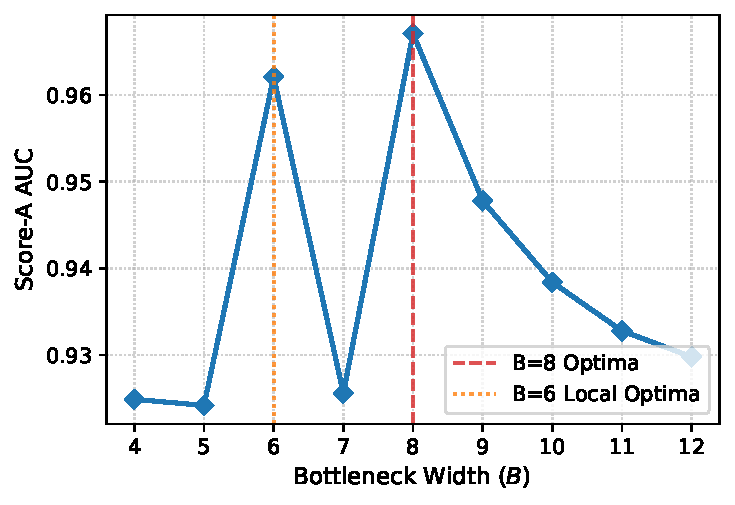
\includegraphics[width=0.85\columnwidth]{ablation_bottleneck.pdf}
\caption{Reconstruction AUC (Score A) as a function of KAN autoencoder bottleneck width $B$. Narrow bottlenecks underfit, while excessive width overfits the healthy manifold and degrades anomaly detection.}
\label{fig:ablation_width}
\end{figure}

\paragraph*{Score comparison.}
The hierarchy of symbolic scores---B ($0.9026\pm0.0558$) $<$
D ($0.9403\pm0.0422$) $<$ M ($\mathbf{0.9891\pm0.0069}$)---reveals
that progressively richer statistical modelling of the healthy
residual distribution yields stronger detectors, while all three
remain fully interpretable. Notably, Score~M achieves the
\textbf{highest mean AUC} across all proposed scores with the
\textbf{lowest variance}, confirming that Mahalanobis whitening
of symbolic residuals is the most robust interpretable detector.
The combined Score~C $(0.5\,\tilde{A}{+}0.5\,\tilde{B})$ achieves
$0.9716\pm0.0151$, demonstrating complementary signal between
symbolic violation and reconstruction error.
Fusing reconstruction with the Mahalanobis score (Score~F,
$0.9824\pm0.0097$) is also highly competitive.

\paragraph*{Fully Symbolic Reconstruction.}
Beyond the first-layer symbolic scores, distilling all layers of the KAN autoencoder into a deep stack of closed-form mathematical equations yields a \emph{fully symbolic reconstruction} score. Across $N{=}10$ seeds this achieves a mean AUC of $\mathbf{0.9777\pm0.0075}$---exceeding the opaque neural network reconstruction (Score~A, $0.9642\pm0.0157$) and placing between the combined Score~C/E ($0.9716$) and Score~F ($0.9824$). Because it entirely replaces the autoencoder with simple mathematical functions, the neural network is completely discarded at inference. Table~\ref{tab:efficiency} quantifies the practical consequence: KAN-AE-SymRecon stores only 10\,889 symbolic scalars---52\% fewer than the KAN-AE's 22\,880 trainable parameters---and runs in \textbf{0.018\,ms} per sample, 
which is $\mathbf{200{\times}}$ faster than SHAP-weighted reconstruction (3.67\,ms; 200 background samples) and $\mathbf{271{\times}}$ faster than LIME-weighted reconstruction (4.99\,ms; 300 perturbations). When evaluated in optimised C++ (Eigen-batched primitives with sparse scatter-add routing), the symbolic evaluator closes to within 1.4$\times$ of the neural forward pass (Score~A: 0.013\,ms), confirming that the primary advantage of SymRecon is \emph{model-size} and \emph{interpretability}---the stored artefact is a set of human-readable equations rather than opaque weights.

%------------------------------------------------------------
\section{Discussion}
\label{sec:discussion}

\paragraph*{Why does combining calibrated symbolic violations help?}
The calibrated symbolic-violation score (B, mean AUC~$0.9026\pm0.0558$)
performs well on its own, confirming that BIC-optimal symbolic surrogates
capture meaningful per-equation structure after joint-GAM
calibration aligns the raw edge-level predictions with the
network's hidden activations. When combined with the
reconstruction score (A), the resulting Score~C ($0.9716\pm0.0151$) exceeds
both individual scores, indicating that the symbolic violation
signal and the reconstruction error capture partially orthogonal
aspects of the healthy manifold.
The Mahalanobis detector (M, $\mathbf{0.9891\pm0.0069}$) further
improves over Score~B by exploiting the \emph{covariance structure}
of the residuals rather than treating each equation independently;
its low standard deviation confirms reliable performance across
random seeds.

\paragraph*{Why does the quadratic form dominate?}
Two compounding factors explain the $98.2\%$ quadratic rate,
and it is important to disentangle them rather than
over-interpret the result as a physical law.
\emph{First}, the feature domain is analytically favourable:
because all inputs are scaled to $[0,1]$, every sufficiently
smooth univariate function is uniformly approximatable by a
low-degree polynomial on that compact interval (Weierstrass),
so a quadratic already captures the bulk of any smooth
B-spline without needing exotic primitives.
\emph{Second}, the $L_1$+entropy regulariser of
\texttt{efficient-kan} suppresses high-curvature splines,
producing near-parabolic activation profiles around the
training-data midpoint that further close the gap between the
spline and its quadratic surrogate.
These two modelling choices are sufficient to explain the
observed dominance; no claim is made that gearbox physics is
intrinsically quadratic.
The practical consequence is nevertheless useful: each term
$g_{ji}(x_i)\!=\!a_{ji}x_i^2\!+\!b_{ji}x_i\!+\!c_{ji}$
is a single scalar expression with three interpretable
coefficients that is trivially deployable on a microcontroller
and differentiable in closed form.
Future work on unscaled or multi-machine datasets should test
whether richer primitives emerge when the domain-scaling bias
is removed.

\paragraph*{Comparison to SHAP/LIME.}
Multi-seed evaluation reveals that the single-seed SHAP AUC of $99.49\%$
was an outlier: the mean over ten seeds is $95.35\pm1.29\%$, which falls
\emph{below} Score~M ($98.91\pm0.69\%$), Score~F ($98.24\pm0.97\%$),
and even LIME-weighted reconstruction ($98.21\pm0.76\%$). This variance
in SHAP scores arises from its dependence on random background centroids
and the specific faulty samples explained per seed.
Beyond accuracy, Table~\ref{tab:efficiency} exposes a severe inference-time cost:
computing a SHAP explanation for a single sample requires 3.67\,ms
(200 perturbations) and LIME requires 4.99\,ms
(300 perturbations), versus 0.013\,ms for the opaque KAN-AE forward pass
and 0.018\,ms for the fully symbolic KAN-AE-SymRecon---making SHAP
\textbf{283$\times$} and LIME \textbf{384$\times$} slower than the neural baseline.
Both XAI methods also incur (i)~$\mathcal{O}(k n^2)$ sampling complexity per
explanation, (ii)~no physical equation, and (iii)~no
localisation: the ten most important SHAP features
(\{S1\_rms, S1\_std, S4\_mean, \ldots\}) and the ten most
important LIME features (\{S3\_rms, S3\_std, S4\_std,
\ldots\}) overlap on only \emph{two} features (S3\_std and S2\_std). In
contrast, Score~M returns a sparse vector of 22 equation
residuals that are reproducible, require no external explainer
at inference, and are directly mappable to specific sensor statistics.

\paragraph*{Limitations.}
(i) Our evaluation uses a single fault mode (broken tooth).
Validating the symbolic equations on bearing-wear and
misalignment datasets is future work.
(ii) Although the symbolic library already includes thirteen
primitives (including piecewise and oscillatory forms), only
five types were selected on this dataset; exploring
data-driven library construction could improve flexibility.
(iii) While our framework successfully symbolises the entire
autoencoder (yielding a fully symbolic reconstruction AUC
of $0.9777\pm0.0075$ that requires no neural network at inference),
we restrict our interpretability analysis to the first layer.
Extracting physical meaning from the deeply composed
formulas remains an open challenge.

%------------------------------------------------------------
\section{Conclusion}
\label{sec:conclusion}

We presented a fully unsupervised framework that turns a
Kolmogorov--Arnold autoencoder into a bank of closed-form
\emph{health equations} for gearbox fault detection.
By distilling each first-layer B-spline edge into a
BIC-optimal symbolic primitive, we obtain 22 human-readable
equations that describe the healthy operating manifold with
a mean $R^2$ of 0.9999. Anomalies are detected through
multiple complementary symbolic scores (mean\,$\pm$\,std over
$N{=}10$ seeds): the calibrated symbolic-violation detector
achieves an AUC of $0.9026\pm0.0558$, and the Mahalanobis
symbolic-residual detector reaches \textbf{$0.9891\pm0.0069$}---the
highest mean and lowest variance of all proposed scores,
surpassing OC-SVM ($0.9856\pm0.0038$), SHAP-weighted reconstruction
($0.9535\pm0.0129$), and all deep baselines, while remaining fully
interpretable and second only to LOF ($0.9937\pm0.0025$).
The combined reconstruction + calibrated symbolic
detector attains AUC $0.9716\pm0.0151$,
exceeding the opaque reconstruction score ($0.9642\pm0.0157$) and the
majority of unsupervised baselines. Unlike SHAP/LIME explanations---which
achieve only $0.9535\pm0.0129$ and $0.9821\pm0.0076$ respectively in the
multi-seed evaluation, with high variance from random background
sampling---the proposed health equations are available in closed form,
require no re-running of an explainer at inference, and
provide a principled route from a violated equation to the
specific sensor statistics that deviated under fault. Furthermore, by symbolising the entire
autoencoder into a stack of simple mathematical equations, we achieve a
\emph{fully symbolic reconstruction} AUC of $0.9777\pm0.0075$ using only
10\,889 stored symbolic scalars (52\% fewer than the KAN-AE's
22\,880 trainable parameters), with a per-sample inference time of
0.018\,ms---200$\times$ faster than SHAP and 271$\times$ faster than
LIME---entirely discarding the neural network at deployment.
These properties make KAN-symbolic health equations a promising ingredient for
trustworthy, deployable condition monitoring of rotating
machinery.

%------------------------------------------------------------
\bibliographystyle{IEEEtran}
\begin{thebibliography}{00}

\bibitem{lei2020}
Y.~Lei, B.~Yang, X.~Jiang, F.~Jia, N.~Li, A.~K. Nandi:
Applications of machine learning to machine fault diagnosis: A review and roadmap.
\textit{Mech.\ Syst.\ Signal Process.}\ \textbf{138}, 106587 (2020).
\href{https://doi.org/10.1016/j.ymssp.2019.106587}{doi:10.1016/j.ymssp.2019.106587}

\bibitem{liu2024kan}
Z.~Liu, Y.~Wang, S.~Vaidya, F.~Ruehle, J.~Halverson, M.~Solja\v{c}i\'c,
T.~Y.~Hou and M.~Tegmark,
``KAN: Kolmogorov--Arnold Networks,''
\emph{arXiv:2404.19756}, 2024.

\bibitem{vaca2024kolmogorov}
R.~Vaca-Rubio, L.~Blanco, R.~Pereira and M.~Caus,
``Kolmogorov--Arnold Networks (KANs) for time series analysis,''
\emph{arXiv:2405.08790}, 2024.

\bibitem{IsolationForest}
F.~T.~Liu, K.~M.~Ting, and Z.-H.~Zhou,
``Isolation forest,''
in \emph{Proc.\ IEEE Int.\ Conf.\ Data Mining (ICDM)}, 2008, pp.\ 413--422.

\bibitem{OCSVM}
B.~Sch\"olkopf, J.~C.~Platt, J.~Shawe-Taylor, A.~J.~Smola, and R.~C.~Williamson,
``Estimating the support of a high-dimensional distribution,''
\emph{Neural Computation}, vol.~13, no.~7, pp.\ 1443--1471, 2001.

\bibitem{LOF}
M.~M.~Breunig, H.-P.~Kriegel, R.~T.~Ng, and J.~Sander,
``LOF: Identifying density-based local outliers,''
in \emph{Proc.\ ACM SIGMOD Int.\ Conf.\ Management of Data}, 2000, pp.\ 93--104.

\bibitem{patchcoreref}
K.~Roth, L.~Pemula, J.~Zepeda, B.~Sch\"olkopf, T.~Brox, and P.~Gehler,
``Towards total recall in industrial anomaly detection,''
in \emph{Proc.\ CVPR}, 2022.

\bibitem{autoencref}
G.~E.~Hinton and R.~R.~Salakhutdinov,
``Reducing the dimensionality of data with neural networks,''
\emph{Science}, vol.~313, no.~5786, pp.\ 504--507, 2006.

\bibitem{vaeref}
D.~P.~Kingma and M.~Welling,
``Auto-encoding variational Bayes,''
in \emph{Proc.\ Int.\ Conf.\ Learning Representations (ICLR)}, 2014.

\bibitem{deeponeclassref}
L.~Ruff \emph{et al.},
``Deep one-class classification,''
in \emph{Proc.\ ICML}, 2018.

\bibitem{teacherstudent}
P.~Bergmann, M.~Fauser, D.~Sattlegger and C.~Steger,
``Uninformed students: Student--teacher anomaly detection
with discriminative latent embeddings,''
in \emph{Proc.\ CVPR}, 2020.
\bibitem{ssldaeref}
P.~Vincent, H.~Larochelle, Y.~Bengio, and P.-A.~Manzagol,
``Extracting and composing robust features with denoising autoencoders,''
in \emph{Proc.\ Int.\ Conf.\ Machine Learning (ICML)}, 2008, pp.\ 1096--1103.

\bibitem{shapref}
S.~M.~Lundberg and S.-I.~Lee,
``A unified approach to interpreting model predictions,''
in \emph{Proc.\ Advances in Neural Information Processing Systems (NeurIPS)},
vol.~30, 2017.

\bibitem{LIMEref}
M.~T.~Ribeiro, S.~Singh, and C.~Guestrin,
```Why should I trust you?': Explaining the predictions of any classifier,''
in \emph{Proc.\ ACM SIGKDD Int.\ Conf.\ Knowledge Discovery and Data Mining},
2016, pp.\ 1135--1144.

\bibitem{Mahalanobis1ref}
X.~Zhao, Z.~Zhao, X.~Cui \emph{et al.},
``Few-shot bearing fault diagnosis using adaptive detail convolution and
global KAN-transformer with Mahalanobis distance,''
\emph{J.\ Vib.\ Eng.\ Technol.}, vol.~13, no.~296, 2025.

\bibitem{Mahalanobis2ref}
Y.~Hou, Z.~Chen, M.~Wu, C.-S.~Foo, X.~Li, and R.~M.~Shubair,
``Mahalanobis distance based adversarial network for anomaly detection,''
in \emph{Proc.\ IEEE Int.\ Conf.\ Acoustics, Speech and Signal Processing
(ICASSP)}, Barcelona, Spain, 2020, pp.\ 3192--3196.

\bibitem{Mahalanobis3ref}
R.~Kamoi and K.~Kobayashi,
``Why is the Mahalanobis distance effective for anomaly detection?''
\emph{arXiv preprint arXiv:2003.00402}, 2020.

\bibitem{cranmer2020discovering}
M.~Cranmer \emph{et al.},
``Discovering symbolic models from deep learning with
inductive biases,''
in \emph{Proc.\ NeurIPS}, 2020.

\bibitem{spectraquest}
I.~U.~Hassan, K.~Panduru, D.~Riordan and J.~Walsh,
``A moving window-based feature extraction method for
gearbox fault detection using vibration signals,''
\emph{Machines}, vol.~14, no.~2, p.~178, 2026.

\end{thebibliography}

\end{document}
